% Final report for the Robust-Overfitting project.
% Compile from the report directory so the figure paths resolve as written.
\documentclass[11pt]{article}

\usepackage[margin=1in]{geometry}
\usepackage[T1]{fontenc}
\usepackage[utf8]{inputenc}
\usepackage{lmodern}
\usepackage[nopatch=footnote]{microtype}
\usepackage{amsmath,amssymb}
\usepackage{booktabs}
\usepackage{tabularx}
\usepackage{multirow}
\usepackage{graphicx}
\usepackage{caption}
\usepackage{placeins}
\usepackage{needspace}
\captionsetup[table]{position=top,skip=0.55em}
\makeatletter
\setlength{\@fptop}{0pt}
\setlength{\@fpsep}{18pt plus 2pt minus 2pt}
\setlength{\@fpbot}{0pt plus 1fil}
\makeatother
\usepackage{xcolor}
\usepackage{hyperref}
\usepackage[nameinlink,capitalise]{cleveref}
\usepackage{enumitem}
\usepackage{setspace}

\hypersetup{
  colorlinks=true,
  linkcolor=blue!55!black,
  citecolor=blue!55!black,
  urlcolor=blue!55!black,
  pdftitle={Robust Overfitting Across Pixel-Space and Low-Frequency Adversarial Training}
}
\setlength{\emergencystretch}{2em}
\setlist[itemize]{leftmargin=*,nosep}
\setlist[enumerate]{leftmargin=*,nosep}

\newcommand{\method}[1]{\textsc{#1}}
\newcommand{\acc}{\mathrm{Acc}}
\newcommand{\linf}{\ell_\infty}
\newcommand{\E}{\mathcal{E}}

\title{Robust Overfitting Across Pixel-Space and Low-Frequency Adversarial Training}
\author{Kaiwen Du\\
  \normalsize Department of Mathematics and Computer Science\\
  \normalsize Santa Clara University}
\date{September 2026}

\begin{document}
\maketitle

\begin{abstract}
Adversarial training can improve robustness to bounded input perturbations, but
its robust test performance may peak and then degrade as training continues, a
phenomenon known as robust overfitting. This report studies how the perturbation
domain used during adversarial training affects that trajectory. We train
PreActResNet-18 models on CIFAR-10 for 200 epochs under pixel-only,
low-frequency-only, and epoch-wise mixed-domain projected gradient descent
(PGD) training. Each condition is evaluated across five seeds using four accuracy metrics:
clean, pixel-PGD-20, low-frequency DCT-masked PGD-20, and joint. Joint accuracy
is the percentage of test images correctly classified under each of two
separately generated attacks. Under pixel-only training, mean pixel robustness peaked at 51.22\%
at epoch 105 and fell by 8.56 percentage points by epoch 200. In contrast,
matched-domain robustness under low-frequency-only training declined by just
0.05 points from its 92.74\% peak, although pixel and joint accuracy
remained at 0.00\%. Mixed-domain training produced schedule-dependent
oscillations: mean pixel robustness was 42.36\% after pixel-training epochs
and 3.53\% after low-frequency-training epochs. These results show that the
observed robust-overfitting trajectory depends strongly on the perturbation
domain and that once-per-epoch random mixing yields domain-specialized states
rather than stable robustness across both evaluated attacks.
\end{abstract}

\section{Introduction}
\label{sec:introduction}

Deep neural networks can be highly accurate on unmodified images while being
vulnerable to small, deliberately chosen perturbations
\cite{goodfellow2015,rice2020}. Adversarial training addresses this threat by
optimizing a model on adversarially perturbed examples. However, robust
performance need not improve monotonically: robust test accuracy can peak and
then decline even as robust training loss continues to decrease. Rice
et al.~\cite{rice2020} describe this phenomenon as robust overfitting; Yu
et al.~\cite{yu2022} further investigate its causes. This gap between the best and
final robust checkpoint is the practical and empirical focus of this study.

To study robust overfitting, we must specify which perturbations the training
and evaluation attacks can use. Standard pixel-space PGD
can change every image coordinate within an $\linf$ budget, whereas a
frequency-restricted attack constrains its perturbation to smooth,
low-frequency patterns. Prior work links frequency content to robust features
and shows that robustness can trade off across heterogeneous perturbation
models \cite{guo2020,bu2023,tramer2019,maini2020}. We therefore examine how the training attack affects when robust test accuracy
peaks and how far it subsequently declines under each evaluation attack.

\paragraph{Research question.}
During PGD adversarial training of PreActResNet-18 on CIFAR-10, how does
independently selecting pixel-space or low-frequency DCT-masked PGD with equal
probability at the start of each epoch affect the timing and severity of robust
overfitting, compared with training exclusively against either attack?

\paragraph{Hypothesis.}
With architecture, dataset, optimization schedule, perturbation budget, and
checkpoint-evaluation schedule held fixed, mixed-domain training will produce
robust-accuracy curves that differ from those of the single-domain conditions. In
particular, the peak epoch, peak shape, or post-peak decline may change under
pixel-space and/or low-frequency evaluation.

\paragraph{Contributions.}
This report makes the following scoped contributions:
\begin{itemize}
  \item It implements and evaluates three controlled adversarial-training
  conditions using standard pixel PGD, DCT-masked low-frequency PGD, or a
  seeded epoch-wise choice between them.
  \item It tracks each saved checkpoint under clean, pixel-PGD-20,
  low-frequency-PGD-20, and per-example joint evaluation, rather than
  reporting only the threat model used for training.
  \item It measures when robust test accuracy peaks and how far it declines
  by the final checkpoint across five seeds for each condition.
  \item It shows that once-per-epoch random domain mixing yields
  schedule-dependent domain specialization under the specified finite-step
  evaluations, rather than stable simultaneous robustness to both attacks.
\end{itemize}

\section{Background and Related Work}
\label{sec:related-work}

\subsection{Adversarial examples and PGD adversarial training}
For a classifier $f_\theta$, input $x$, label $y$, and loss
$\ell(f_\theta(x),y)$, an $\linf$ adversary seeks a perturbation $\delta$
that increases loss while satisfying $\lVert\delta\rVert_\infty\leq\epsilon$.
Fast gradient sign attacks use a single gradient step; PGD repeats projected
gradient ascent, often from a random start, to form a stronger first-order
attack \cite{goodfellow2015,madry2018}. In adversarial training, the model is
optimized on such attacked examples rather than treating the attack only as a
post-hoc evaluation.

We use PGD-10 during training to keep the cost of adversarial-example
generation manageable across 200 epochs, while PGD-20 allocates more attack
iterations to the primary checkpoint evaluation. The additional iterations
are intended to provide a more thorough finite-step search under the same
perturbation budget, but they do not guarantee a worst-case perturbation or
certify robustness.

\subsection{Robust overfitting}
Rice et al.~\cite{rice2020} documented robust overfitting across data sets and
threat models: robust test performance can improve near a learning-rate change
and subsequently fall despite continued training. They emphasize selection of
an early checkpoint using a held-out validation set. Yu et al.~\cite{yu2022}
further connect robust overfitting to the treatment of small-loss adversarial
examples. For each robustness metric, we measure the decline from its highest observed
test accuracy to its accuracy at epoch 200; \cref{sec:overfitting-measures}
defines the peak epoch and peak-to-final accuracy gap used in this study.

\subsection{Frequency-restricted and multi-threat robustness}
The discrete cosine transform (DCT) represents images with spatial-frequency
coefficients. Restricting a perturbation to low-frequency coefficients produces
smooth, broad image changes \cite{guo2020}. Frequency-aware work suggests that
frequency components can make different contributions to prediction and robust
learning \cite{chen2022,bu2023}. Meanwhile, robustness against multiple
perturbation models can be imbalanced: a model trained for one threat may
remain weak for another \cite{tramer2019,maini2020}. Recent work also relates
heterogeneous threat models to distinct spectral signatures and possible
negative transfer \cite{xie2026}.

Tram\`er and Boneh generate an adversarial example from each threat model for
every training input. AVG trains on all of these examples, whereas MAX trains
only on the example with the highest loss \cite{tramer2019}. Maini
et al.'s Multi Steepest Descent (MSD) instead incorporates the threat-model
choice into the inner maximization by selecting the highest-loss candidate
direction at every attack step \cite{maini2020}. We instead use a
seeded random choice to select pixel-space or low-frequency PGD once per
epoch. Every batch in that epoch uses the selected attack. This alternates
between two training objectives across epochs, without selecting the
worst-case attack for each training example.

\section{Methods}
\label{sec:methods}

\subsection{Notation and threat models}
Let $x\in[0,1]^{3\times32\times32}$ denote a color image with three channels
and pixel values scaled to $[0,1]$, and let $y\in\{1,\ldots,10\}$ denote its
class label. A perturbation $\delta$ is an additive change to the image. We
use a perturbation budget of $\epsilon=8/255$, which limits the maximum
absolute change to any pixel-channel value.
We define the perturbation-budget set and the pixel-space threat set as
\[
\begin{aligned}
\mathcal{B}_\infty(\epsilon)
  &=\{\delta:\lVert\delta\rVert_\infty\leq\epsilon\},\\
\mathcal{S}_x
  &=\{\delta\in\mathcal{B}_\infty(\epsilon):
      x+\delta\in[0,1]^{3\times32\times32}\}.
\end{aligned}
\]
The set $\mathcal{B}_\infty(\epsilon)$ contains perturbations within this
budget. The pixel-space threat set $\mathcal{S}_x$ additionally requires the
perturbed image to remain within $[0,1]$.
The low-frequency threat model
applies a two-dimensional DCT to the perturbation, retains an $8\times8$
top-left block of coefficients per channel, and transforms the result back to
pixel space. Thus it retains $64$ of the $1{,}024$ coefficients per channel
before the final image-range clipping step.

The low-frequency projection used in the implementation is
\begin{equation}
  P_8(\delta)=C^\top\bigl(M_8\odot(C\delta C^\top)\bigr)C.
  \label{eq:dct-projection}
\end{equation}
Here, $C$ is the $32\times32$ orthonormal DCT-II matrix, $C^\top$ is its
transpose, and $\odot$ denotes element-wise multiplication. The mask $M_8$
is one inside the top-left $8\times8$ block and zero elsewhere. The
projection $P_8$ is applied separately to each color channel.
The code uniformly rescales projected perturbations when necessary to enforce
the $\linf$ budget, rather than clipping individual perturbation coordinates;
the resulting image is then clipped to $[0,1]$.

\Needspace{12\baselineskip}
\subsection{Attack generation}
\label{sec:attacks}
For pixel-space PGD, the attack begins from a uniformly random perturbation in
the $\linf$ ball, clips the perturbed image to $[0,1]$, and iterates
\begin{equation}
  \delta_{t+1}=\Pi_{\mathcal{S}_x}
  \left(\delta_t+\alpha\,\mathrm{sign}\left(\nabla_\delta
  \ell(f_\theta(x+\delta_t),y)\right)\right),
  \qquad \alpha=2/255.
  \label{eq:pixel-pgd}
\end{equation}
Here, $\delta_t$ is the perturbation at attack step $t$, and $\alpha$ is the
step size. The gradient $\nabla_\delta\ell$ describes how the loss changes
with the perturbation, and $\mathrm{sign}$ takes its element-wise sign. The
projection $\Pi_{\mathcal{S}_x}$ clips the updated perturbation to satisfy
both the perturbation budget and the valid image range.

For low-frequency PGD, the random start and gradient direction are projected
with $P_8$. The projected direction is normalized by its per-example maximum
absolute value before its $\alpha$-sized update, then the perturbation is
uniformly rescaled if it exceeds $\epsilon$. At every step, the loss is
computed on the image clipped to $[0,1]$, while the stored low-frequency
perturbation remains unclipped. Both attacks are white-box, untargeted
cross-entropy attacks; $f_\theta$ includes the input normalization described
below. Attack generation uses evaluation-mode BatchNorm statistics.
Each primary evaluation uses one random start and returns the final iterate.

The implementation checks in Appendix~\ref{app:checks} confirm that the DCT
round-trip and masked projection are numerically accurate before final image
clipping. Clipping to $[0,1]$ does introduce nonzero out-of-mask energy: in a
256-image diagnostic low-frequency-PGD-20 run, its mean fraction was 0.70\%,
with a 95th percentile of 4.75\% and maximum of 17.56\%. We therefore use
``DCT-masked low-frequency PGD'' to describe the attack-generation procedure,
not a claim that every final, image-clipped perturbation is exactly
band-limited. The final perturbations remained within the stated $\linf$
budget to floating-point precision.

\subsection{Training conditions}
\label{sec:conditions}
The pixel-only, low-frequency-only, and mixed-domain conditions share the
model, dataset, optimizer, learning-rate schedule, and perturbation budget
specified below. They differ in how adversarial training examples are
generated. The low-frequency attack changes both the search domain and the
update rule: it uses normalized projected gradients and uniform rescaling,
whereas pixel PGD uses signed gradients and coordinate-wise clipping. The
comparison therefore evaluates these attack procedures together, rather than
isolating frequency restriction from attack optimization.

\begin{table}[htbp]
\centering
\caption{Training conditions. All full experiments use seeds 42--46.}
\label{tab:conditions}
\begin{tabularx}{\linewidth}{@{}lX@{}}
\toprule
Condition & Adversarial examples used for every training batch in an epoch \\
\midrule
Pixel-only & Standard pixel-space PGD-10. \\
Low-frequency-only & DCT-masked low-frequency PGD-10 with cutoff $8$. \\
Mixed-domain & A dedicated, seeded random-number generator selects pixel-space or
low-frequency PGD with equal probability at the start of each epoch; all
batches in that epoch use the selected attack. \\
\bottomrule
\end{tabularx}
\end{table}

Using a separate generator keeps the domain schedule reproducible for a given
seed, regardless of random draws used for data shuffling, augmentation, or
PGD initialization. Checkpoints save the current
domain, the complete domain schedule so far, the seed, and DCT cutoff.
Appendix~\ref{app:schedules} reports the number of epochs assigned to each
attack domain and the domains used at the aggregate pixel-accuracy peak and
final checkpoint.

\Needspace{14\baselineskip}
\subsection{Optimization and implementation details}
\label{sec:implementation}
We use PreActResNet-18, based on the pre-activation residual architecture of
He et al.~\cite{he2016}, with the implementation provided by Rice
et al.~\cite{rice2020}. Models are trained on CIFAR-10
\cite{krizhevsky2009}. Training uses
random $32\times32$ crops with four-pixel padding and random horizontal flips;
test images receive tensor conversion only. Inputs are normalized with CIFAR-10
channel means $(0.4914,0.4822,0.4465)$ and standard deviations
$(0.2471,0.2435,0.2616)$. Optimization uses SGD with momentum $0.9$, initial
learning rate $0.1$, weight decay $5\times10^{-4}$, and MultiStep learning-rate
decays by a factor of $0.1$ after epochs 100 and 150.

\begin{table}[htbp]
\centering
\caption{Experimental configuration reported for the full runs.}
\label{tab:configuration}
\begin{tabularx}{\linewidth}{@{}lX@{}}
\toprule
Item & Setting \\
\midrule
Data set & CIFAR-10: 50,000 training and 10,000 test images \\
Architecture & PreActResNet-18 \\
Full training duration & 200 epochs \\
Seeds & 42, 43, 44, 45, 46 \\
Batch size & 128 \\
Optimizer & SGD, momentum $0.9$, weight decay $5\times10^{-4}$ \\
Learning rate & $0.1$, multiplied by $0.1$ after epochs 100 and 150 \\
Training attacks & PGD-10, $\epsilon=8/255$, $\alpha=2/255$ \\
Evaluation attacks & PGD-20, $\epsilon=8/255$, $\alpha=2/255$ \\
Low-frequency mask & $8\times8$ retained DCT block per channel \\
Checkpoint schedule & Every 5 epochs: 40 checkpoints from 5 through 200 \\
\bottomrule
\end{tabularx}
\end{table}
\FloatBarrier

We used NVIDIA A10 GPUs with 24~GB of memory on cloud instances rented from
Lambda Labs for all full training runs and checkpoint evaluations. The retained TensorBoard logs for all 15 full runs
span 5.83 to 5.91 hours from their first to final scalar event; this is a
logging-time measure, not a complete cloud-billing or end-to-end wall-clock
measure.

For each run, we seed the random-number generators in Python, NumPy, and
PyTorch, including all CUDA devices when available. We set
\texttt{cudnn.deterministic} to \texttt{True} and \texttt{cudnn.benchmark}
to \texttt{False}. We do not enable PyTorch's global
deterministic-algorithms mode. Exact cloud OS, CUDA-driver, Python, PyTorch,
and torchvision versions were not preserved in a run manifest and are not
inferred from the current local checking environment.

\section{Evaluation and Analysis}
\label{sec:analysis-plan}

\subsection{Checkpoint evaluation}
Each saved checkpoint is evaluated on the full CIFAR-10 test set under four
quantities:
\begin{enumerate}
  \item clean accuracy, without an attack;
  \item pixel robust accuracy, after pixel-space PGD-20;
  \item low-frequency robust accuracy, after DCT-masked low-frequency PGD-20;
  \item joint accuracy, which counts an image as correct only when both its
  pixel-PGD-20 version and its separately generated low-frequency-PGD-20
  version are correctly classified.
\end{enumerate}
Cross-entropy loss is additionally recorded for clean, pixel-PGD, and
low-frequency-PGD inputs. Values in the overall CSVs are the arithmetic mean
and sample standard deviation across five seeds at each checkpoint.

Appendix~\ref{app:checks} compares single-start PGD-20 with three-restart PGD-50
on two pixel-only checkpoints using a fixed 256-image subset. This check
covers only pixel-space PGD. We did not perform a corresponding comparison
using more iterations and restarts for low-frequency PGD.

\Needspace{10\baselineskip}
\paragraph{Metric interpretation.}
Joint accuracy measures per-example correctness under both generated
attacks; it does not require a correct clean prediction. We label this metric
``union robustness'' in the CSV files and plot legends.'' It is an empirical two-attack
summary, not exact worst-case accuracy over a threat set. Every final
low-frequency perturbation remains within the pixel $\linf$ threat set even
after image clipping, so the union of the two threat sets is the pixel threat
set itself. Differences between their measured accuracies reflect restricted
search and finite-step attack optimization.

\subsection{Robust-overfitting measures}
\label{sec:overfitting-measures}
Following Rice et al.'s description of robust overfitting \cite{rice2020},
we summarize each robustness trajectory by its peak epoch and its decline
from peak accuracy to epoch 200.
For a given training condition, let $A_m(e)$ denote the mean test accuracy
across five seeds for metric $m$ at checkpoint epoch $e$. The evaluated epochs
are $\E=\{5,10,\ldots,200\}$. We define the peak epoch and robust-overfitting
gap as follows:
\begin{align}
  e_m^* &= \underset{e\in\E}{\arg\max}\;A_m(e), \\
  \mathrm{ROG}_m &= A_m(e_m^*)-A_m(200),
  \label{eq:robust-overfitting-gap}
\end{align}
Here, $e_m^*$ is the evaluated epoch with the highest mean accuracy for
metric $m$; the $\arg\max$ operation selects that epoch. If multiple epochs
share the maximum, we choose the earliest. The robust-overfitting gap,
$\mathrm{ROG}_m$, is the difference in percentage points between this peak
accuracy and the accuracy at epoch 200. Aggregate peaks and ROGs
in \cref{tab:main-results} are calculated
from the condition mean trajectory using unrounded values, whereas
Appendix~\ref{app:per-seed} reports each seed's own earliest peak. For mixed-domain
training, ROG is a descriptive gap that also reflects the attack schedule.
The five-seed summaries use mean $\pm$ sample
standard deviation descriptively; this study does not report confidence
intervals or formal hypothesis tests.

Test-set peaks describe the observed trajectories; they are not
validation-selected early-stopping estimates.

\section{Results}
\label{sec:results}

\Cref{tab:main-results} summarizes checkpoint accuracy across five seeds for
each training condition. The following sections examine the trajectories and
the relationship between mixed-domain performance and the training schedule.

\begin{table}[htbp]
\centering
\caption{Five-seed checkpoint-evaluation results. Panel A reports epoch-200
accuracy (\%) as mean $\pm$ sample standard deviation across seeds. Panel B
reports peak accuracy (\%) and robust-overfitting gaps (ROGs, in percentage
points), calculated from the mean trajectory;
the parenthesized value is the peak epoch, with the earliest checkpoint used
to resolve ties. All evaluations use the finite-step attacks defined in
\cref{sec:attacks}.}
\label{tab:main-results}
\setlength{\tabcolsep}{4pt}
\renewcommand{\arraystretch}{1.12}
\textbf{Panel A: Final accuracy}\par\smallskip
\begin{tabular*}{\linewidth}{@{\extracolsep{\fill}}lrrrr@{}}
\toprule
Condition & Clean & Pixel & Low freq. & Joint \\
\midrule
Pixel-only & $84.40\pm0.09$ & $42.66\pm0.22$ & $76.48\pm0.26$ & $42.66\pm0.22$ \\
Low-frequency-only & $94.28\pm0.22$ & $0.00\pm0.00$ & $92.70\pm0.28$ & $0.00\pm0.00$ \\
Mixed-domain & $90.33\pm3.45$ & $19.33\pm14.28$ & $85.20\pm4.29$ & $19.33\pm14.27$ \\
\bottomrule
\end{tabular*}

\medskip
\textbf{Panel B: Peaks and declines}\par\smallskip
\begin{tabular*}{\linewidth}{@{\extracolsep{\fill}}lrrrr@{}}
\toprule
& \multicolumn{2}{c}{Pixel robustness}
& \multicolumn{2}{c}{Low-frequency robustness} \\
\cmidrule(lr){2-3}\cmidrule(lr){4-5}
Condition & Peak (epoch) & ROG & Peak (epoch) & ROG \\
\midrule
Pixel-only & $51.22$ (105) & $8.56$ & $78.36$ (155) & $1.88$ \\
Low-frequency-only & $0.00$ (5) & $0.00$ & $92.74$ (195) & $0.05$ \\
Mixed-domain & $40.80$ (85) & $21.47$ & $86.92$ (195) & $1.72$ \\
\bottomrule
\end{tabular*}
\end{table}

\FloatBarrier
\subsection{Pixel-only control}
\label{sec:pixel-results}
The pixel-only control displays the expected signature of robust overfitting
under pixel-PGD-20: aggregate pixel robustness peaks at epoch 105 and falls by
8.56 percentage points, from 51.22\% to 42.66\%, by epoch 200. Every seed
reaches its individual pixel-robustness peak at epoch 105. Low-frequency
robustness peaks later, at 78.36\% at epoch 155, and ends at 76.48\%, a smaller
1.88-point decline. Mean pixel robust loss reaches its minimum of 1.291 at
epoch 105 and rises to 3.223 by epoch 200, while the final clean accuracy
remains 84.40\%. Pixel and joint accuracy are nearly identical, indicating
that the additional low-frequency attack identifies few failures beyond those
found by pixel-PGD-20.

\begin{figure}[htbp]
  \centering
  
\includegraphics[width=\linewidth]{pixel-only/overall/po_eval.pdf}
  \caption{Pixel-only five-seed checkpoint evaluation. The left panel shows
  mean clean, pixel-PGD-20, low-frequency-PGD-20, and joint accuracy;
  the right panel shows the corresponding clean and attacked cross-entropy
  losses. Shaded bands denote one sample standard deviation across seeds at
  each of the 40 checkpoints evaluated at five-epoch intervals. Pixel
  robustness peaks at epoch 105 and subsequently declines by 8.56 percentage
  points, while low-frequency robustness declines by 1.88 points from its
  later peak.}
  \label{fig:pixel-eval}
\end{figure}

\begin{figure}[htbp]
  \centering
  
\includegraphics[width=\linewidth]{pixel-only/overall/po_train.pdf}
  \caption{Pixel-only training dynamics averaged across five seeds; shaded
  bands denote one sample standard deviation. The left panel reports training
  and in-training test accuracy, and the right reports training robust loss and
  in-training test loss. Training robustness is measured against the pixel
  PGD-10 attack used for optimization, and the logged test-robust quantity also
  uses pixel-PGD-10. These curves show how accuracy and loss change during training. Their
  robust measurements use PGD-10, while the saved-checkpoint evaluations in
  \cref{fig:pixel-eval} use PGD-20, so the attack settings differ between
  the figures.}
  \label{fig:pixel-training}
\end{figure}

\FloatBarrier
\subsection{Low-frequency-only condition}
\label{sec:low-frequency-results}
Low-frequency accuracy remains high late in training, with little decline
from its peak. Mean low-frequency robustness reaches 92.74\% at epoch 195 and ends
at 92.70\%, a decline of only 0.05 percentage points; its final clean accuracy
is 94.28\%. By contrast, pixel-PGD-20 and joint accuracy are 0.00\% at
every evaluated checkpoint for every seed. Low-frequency robust loss reaches
its minimum of 0.266 at epoch 105 and ends at 0.318. Thus, under these
finite-step evaluations, robustness learned against the restricted attack
does not transfer to the pixel-space attack.

\begin{figure}[htbp]
  \centering
  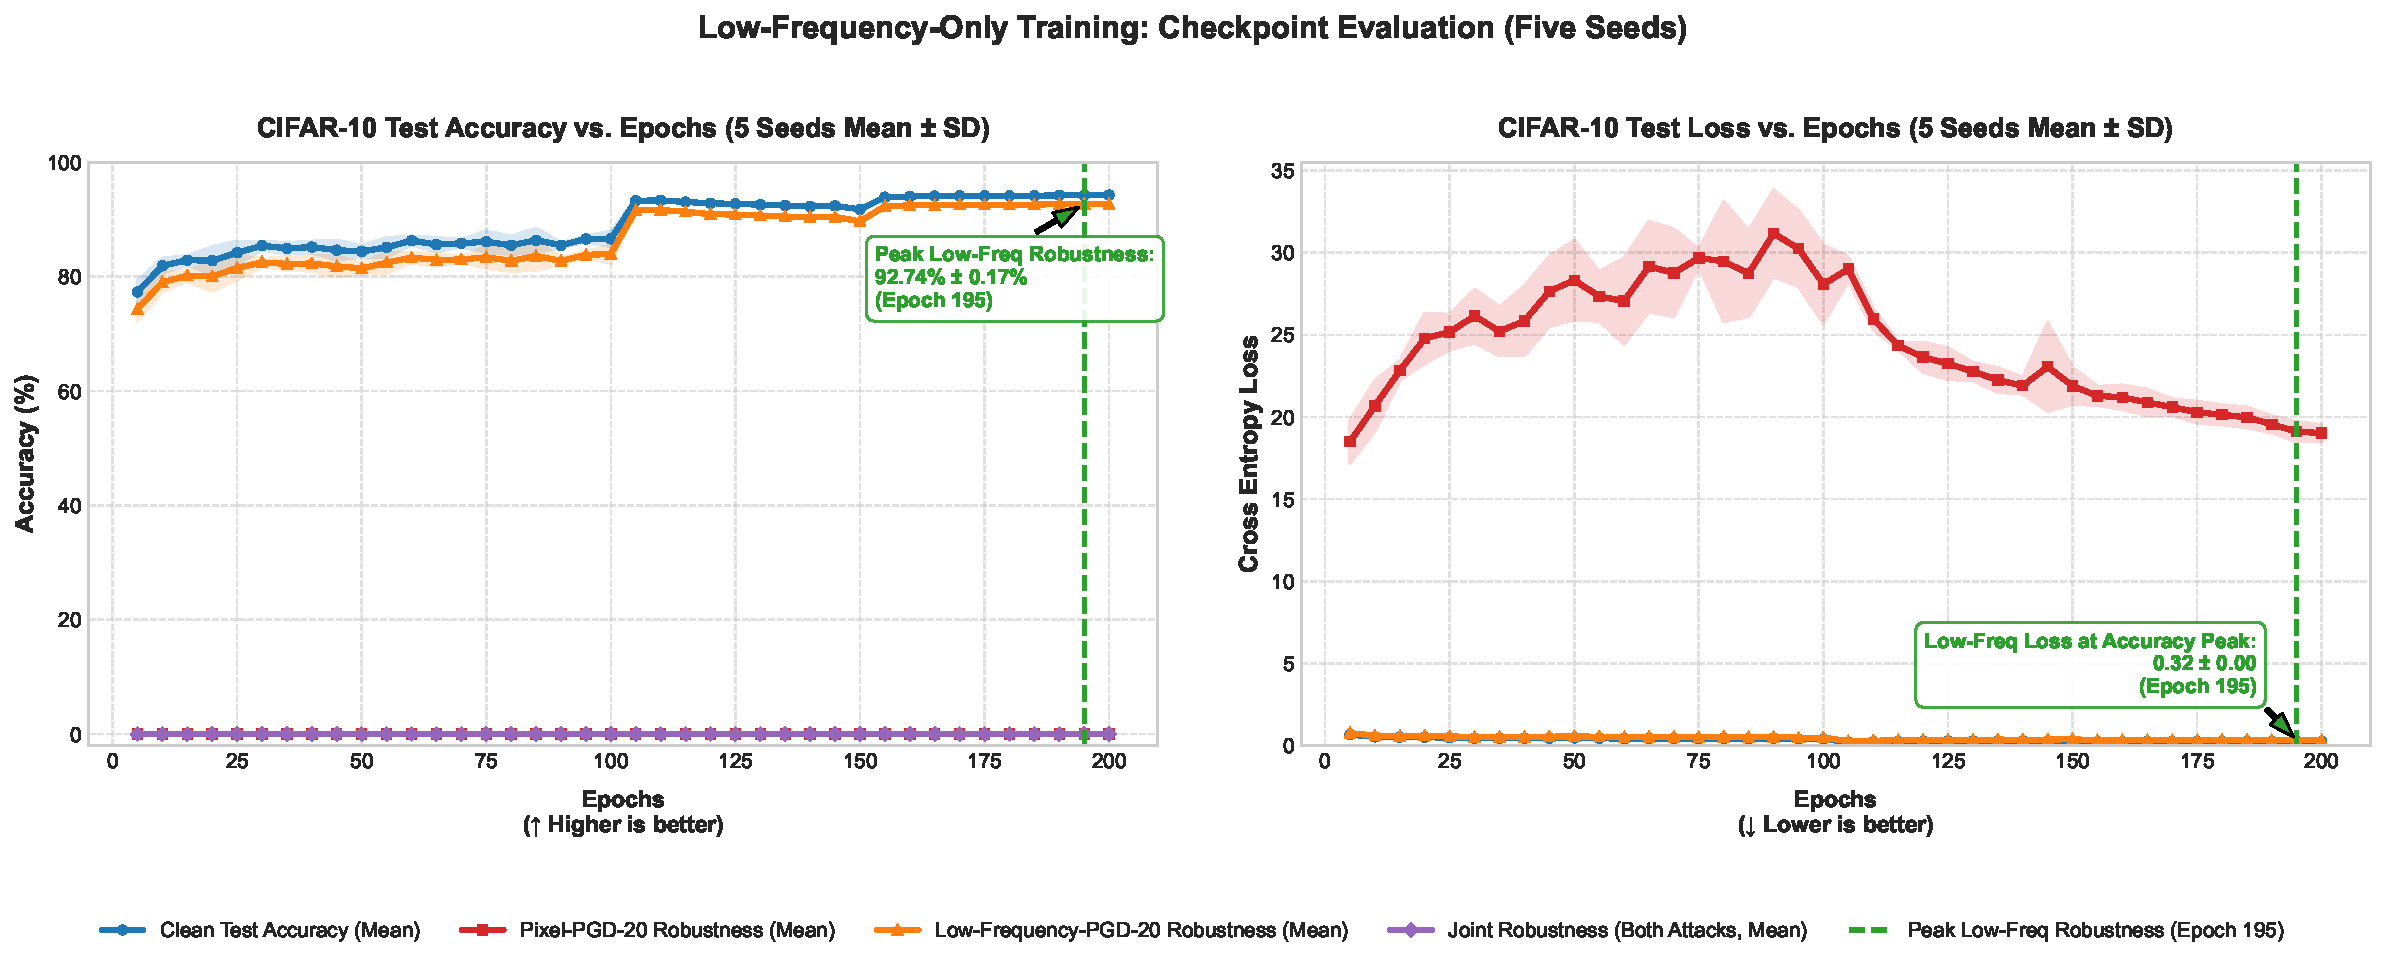
\includegraphics[width=\linewidth]{low-frequency-only/overall/lfo_eval.pdf}
  \caption{Low-frequency-only five-seed checkpoint evaluation, using the same
  panel definitions, checkpoint cadence, and sample-standard-deviation bands
  as \cref{fig:pixel-eval}. Low-frequency-PGD-20 accuracy remains high and
  peaks at 92.74\% at epoch 195, whereas pixel-PGD-20 and joint accuracy
  remain at 0.00\% throughout, showing no measured transfer to pixel-PGD-20.
  The loss annotation reports low-frequency loss at the accuracy peak,
  not the minimum loss, which occurs at epoch 105.}
  \label{fig:lfo-eval}
\end{figure}

\begin{figure}[htbp]
  \centering
  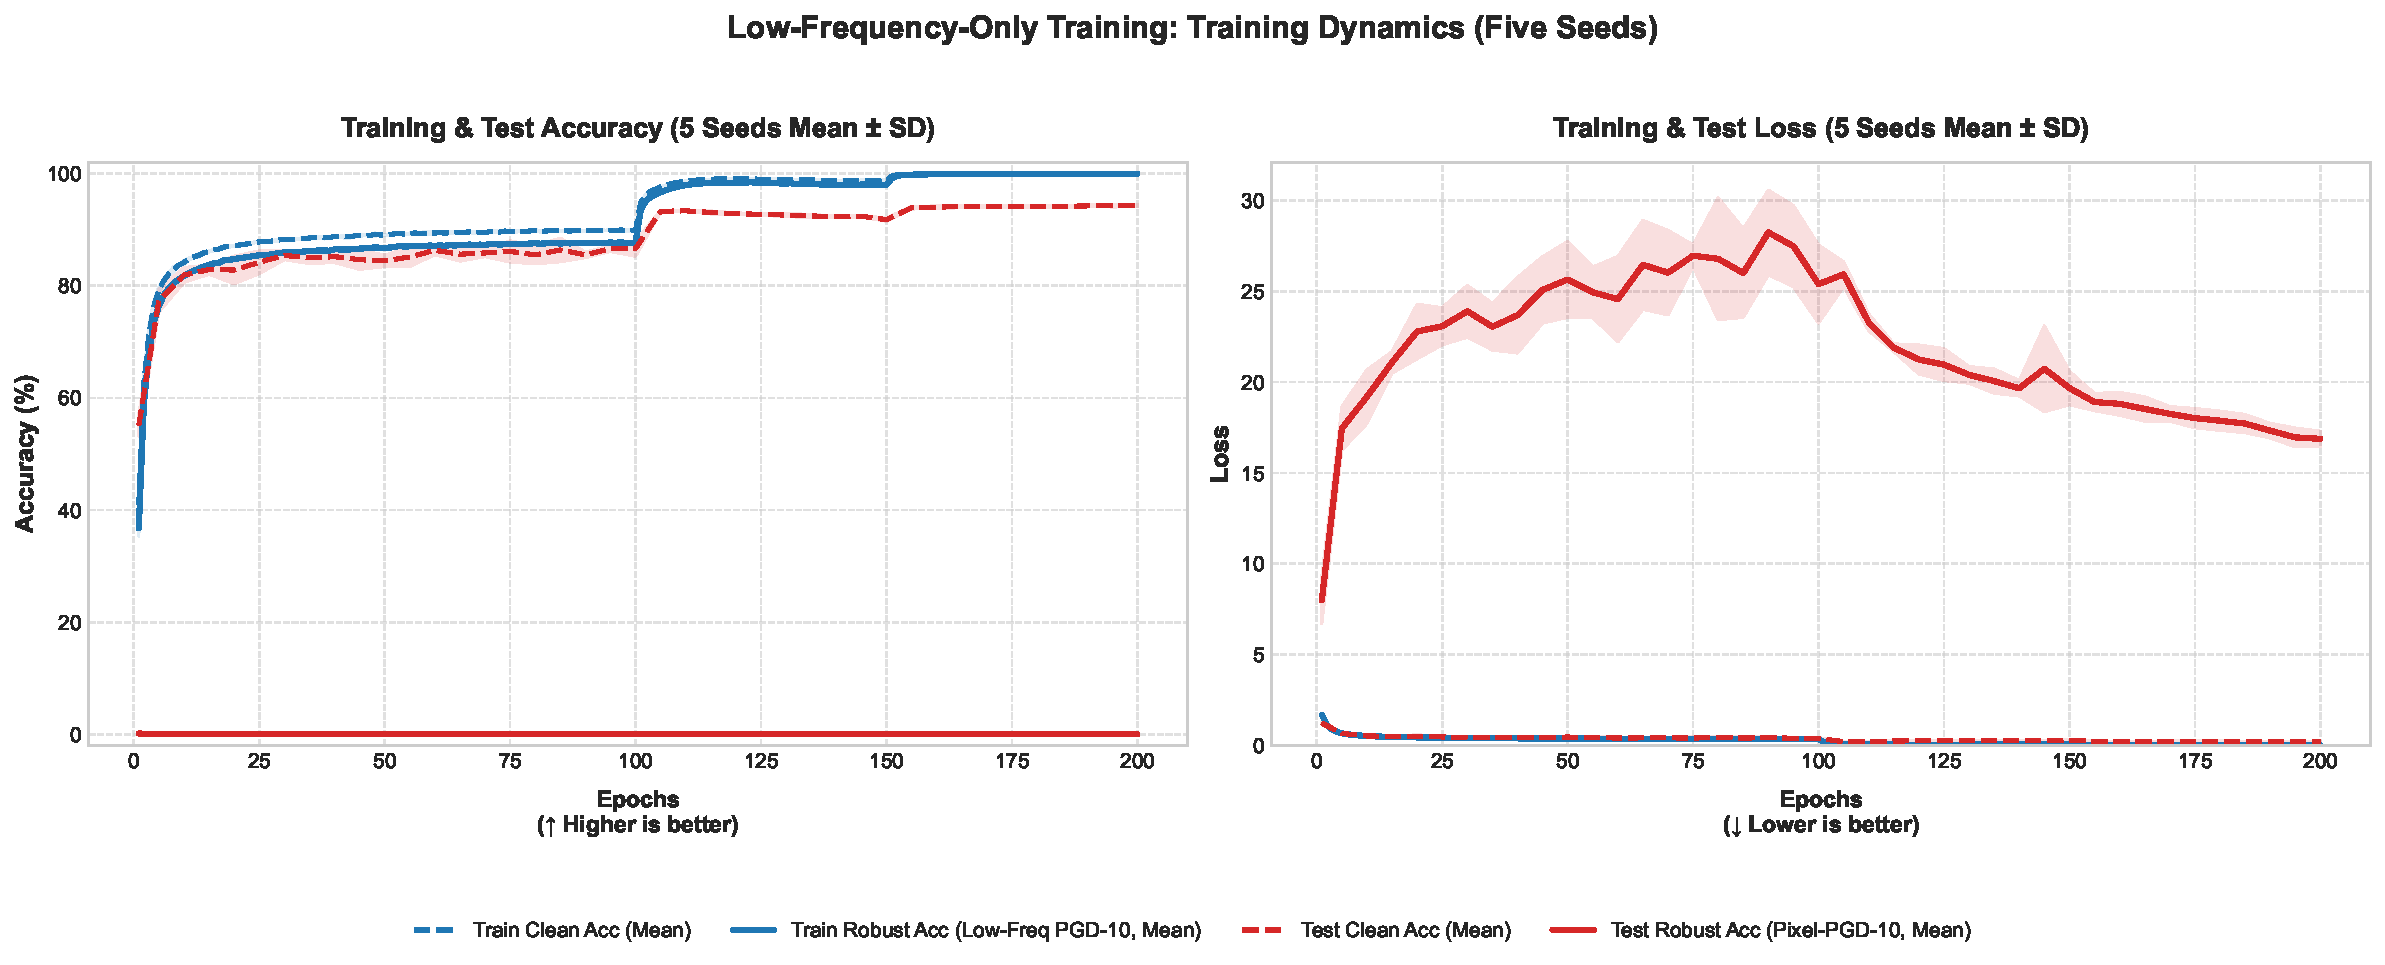
\includegraphics[width=\linewidth]{low-frequency-only/overall/lfo_train.pdf}
  \caption{Low-frequency-only training dynamics averaged across five seeds;
  shaded bands denote one sample standard deviation. Panels and line types
  follow \cref{fig:pixel-training}, but the training robust accuracy and loss
  use the active low-frequency PGD-10 attack. The in-training test-robust curves
  use pixel-PGD-10 in every condition, explaining their sharp contrast with
  the matched-domain training curves and with the low-frequency-PGD-20
  checkpoint results in \cref{fig:lfo-eval}.}
  \label{fig:lfo-training}
\end{figure}

\FloatBarrier
\subsection{Mixed-domain condition}
\label{sec:mixed-results}
The mixed-domain condition yields an aggregate pixel-robustness peak
of 40.80\% and joint peak of 40.79\% at epoch 85. By epoch 200, these
metrics fall to 19.33\% and 19.33\%, respectively, corresponding to raw gaps
of 21.47 and 21.46 percentage points. These peak-to-final gaps also reflect changes in the training attack, so
they cannot be attributed to robust overfitting alone. All five seeds used pixel training at epoch 85,
whereas only seed 42 used pixel training at epoch 200. Across the 200
seed--checkpoint observations, mean pixel robustness is 42.36\% immediately
after pixel-training epochs and 3.53\% after low-frequency-training epochs;
the point-biserial correlation is $r=0.971$, coding pixel training as 1
and low-frequency training as 0. These pooled observations comprise 102
pixel-training and 98 low-frequency-training checkpoints and include repeated
measurements from each seed; the correlation is descriptive and does not
adjust for epoch or training history. Individual seeds reach their joint
peaks between epochs 115 and 160, not at the aggregate peak of epoch 85.

This schedule dependence is also consistent with the large epoch-200 variation:
pixel-PGD-20 and joint accuracy have sample standard deviations of
14.28 and 14.27 percentage points. Low-frequency robustness is higher and
more stable in aggregate, peaking at 86.92\% at epoch 195 and ending at
85.20\%. These results show a strong association between measured robustness
and the most recent training attack. The 21.46-point joint-accuracy gap
therefore cannot be interpreted as robust overfitting alone.

\Cref{fig:mixed-eval} shows the aggregate checkpoint trajectories. To examine
their schedule dependence, we group checkpoint results by the attack used
during the checkpoint's final training epoch
(\cref{fig:mixed-eval-grouped}). The training dynamics are shown separately
in Appendix~\ref{app:mixed-training}.

\begin{figure}[htbp]
  \centering
  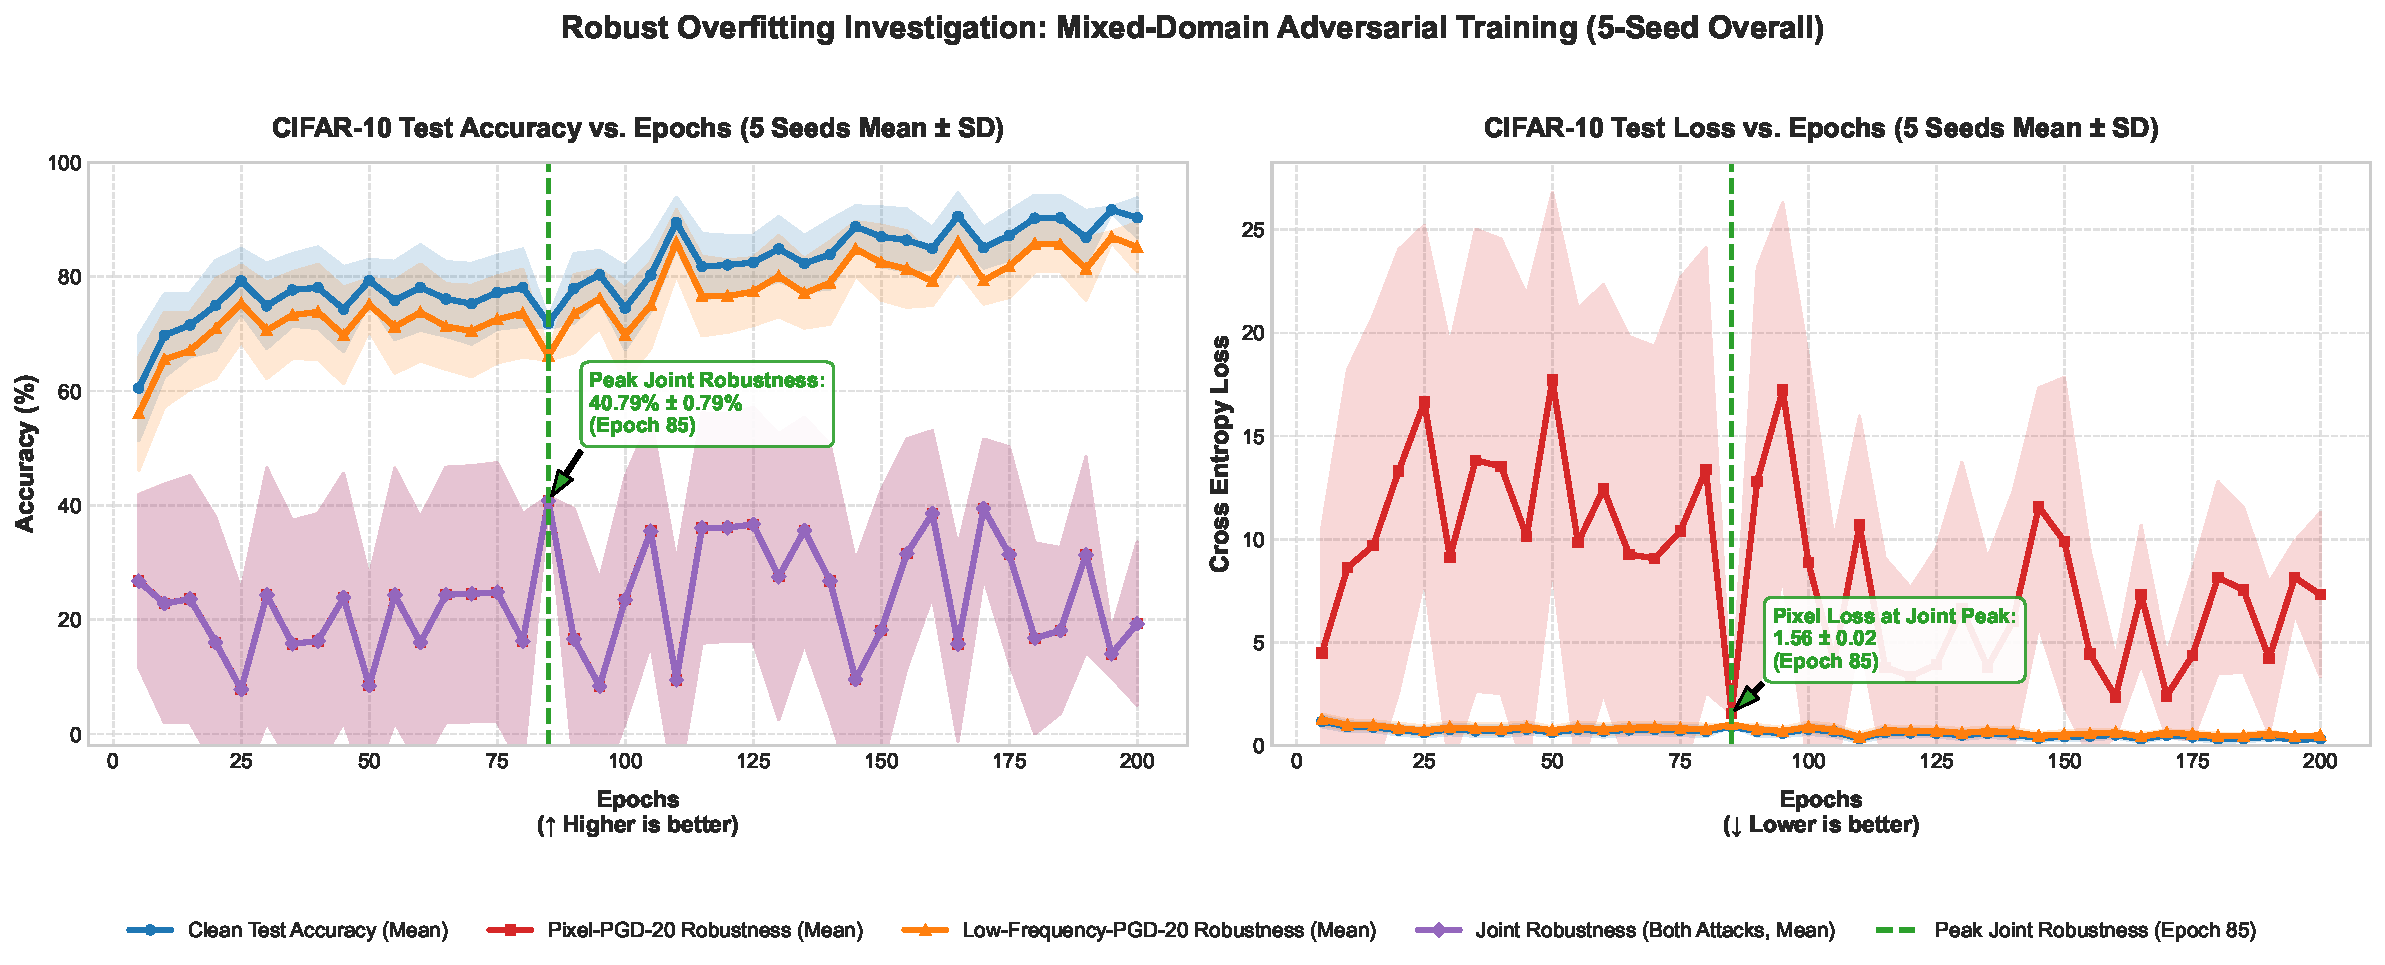
\includegraphics[width=\linewidth]{mixed-domain/overall/mdo_eval.pdf}
  \caption{Mixed-domain five-seed checkpoint evaluation. The left panel shows
  mean clean, pixel-PGD-20, low-frequency-PGD-20, and joint accuracy; the right
  panel shows clean and attacked cross-entropy losses. Shaded bands denote one
  sample standard deviation across seeds. Pixel and joint accuracy peak at
  epoch 85, when all five seeds used pixel training. Their fluctuations and
  peak-to-final gaps also reflect changes in the training attack. The loss
  annotation reports pixel loss at the joint-accuracy peak.}
  \label{fig:mixed-eval}
\end{figure}

\begin{figure}[htbp]
  \centering
  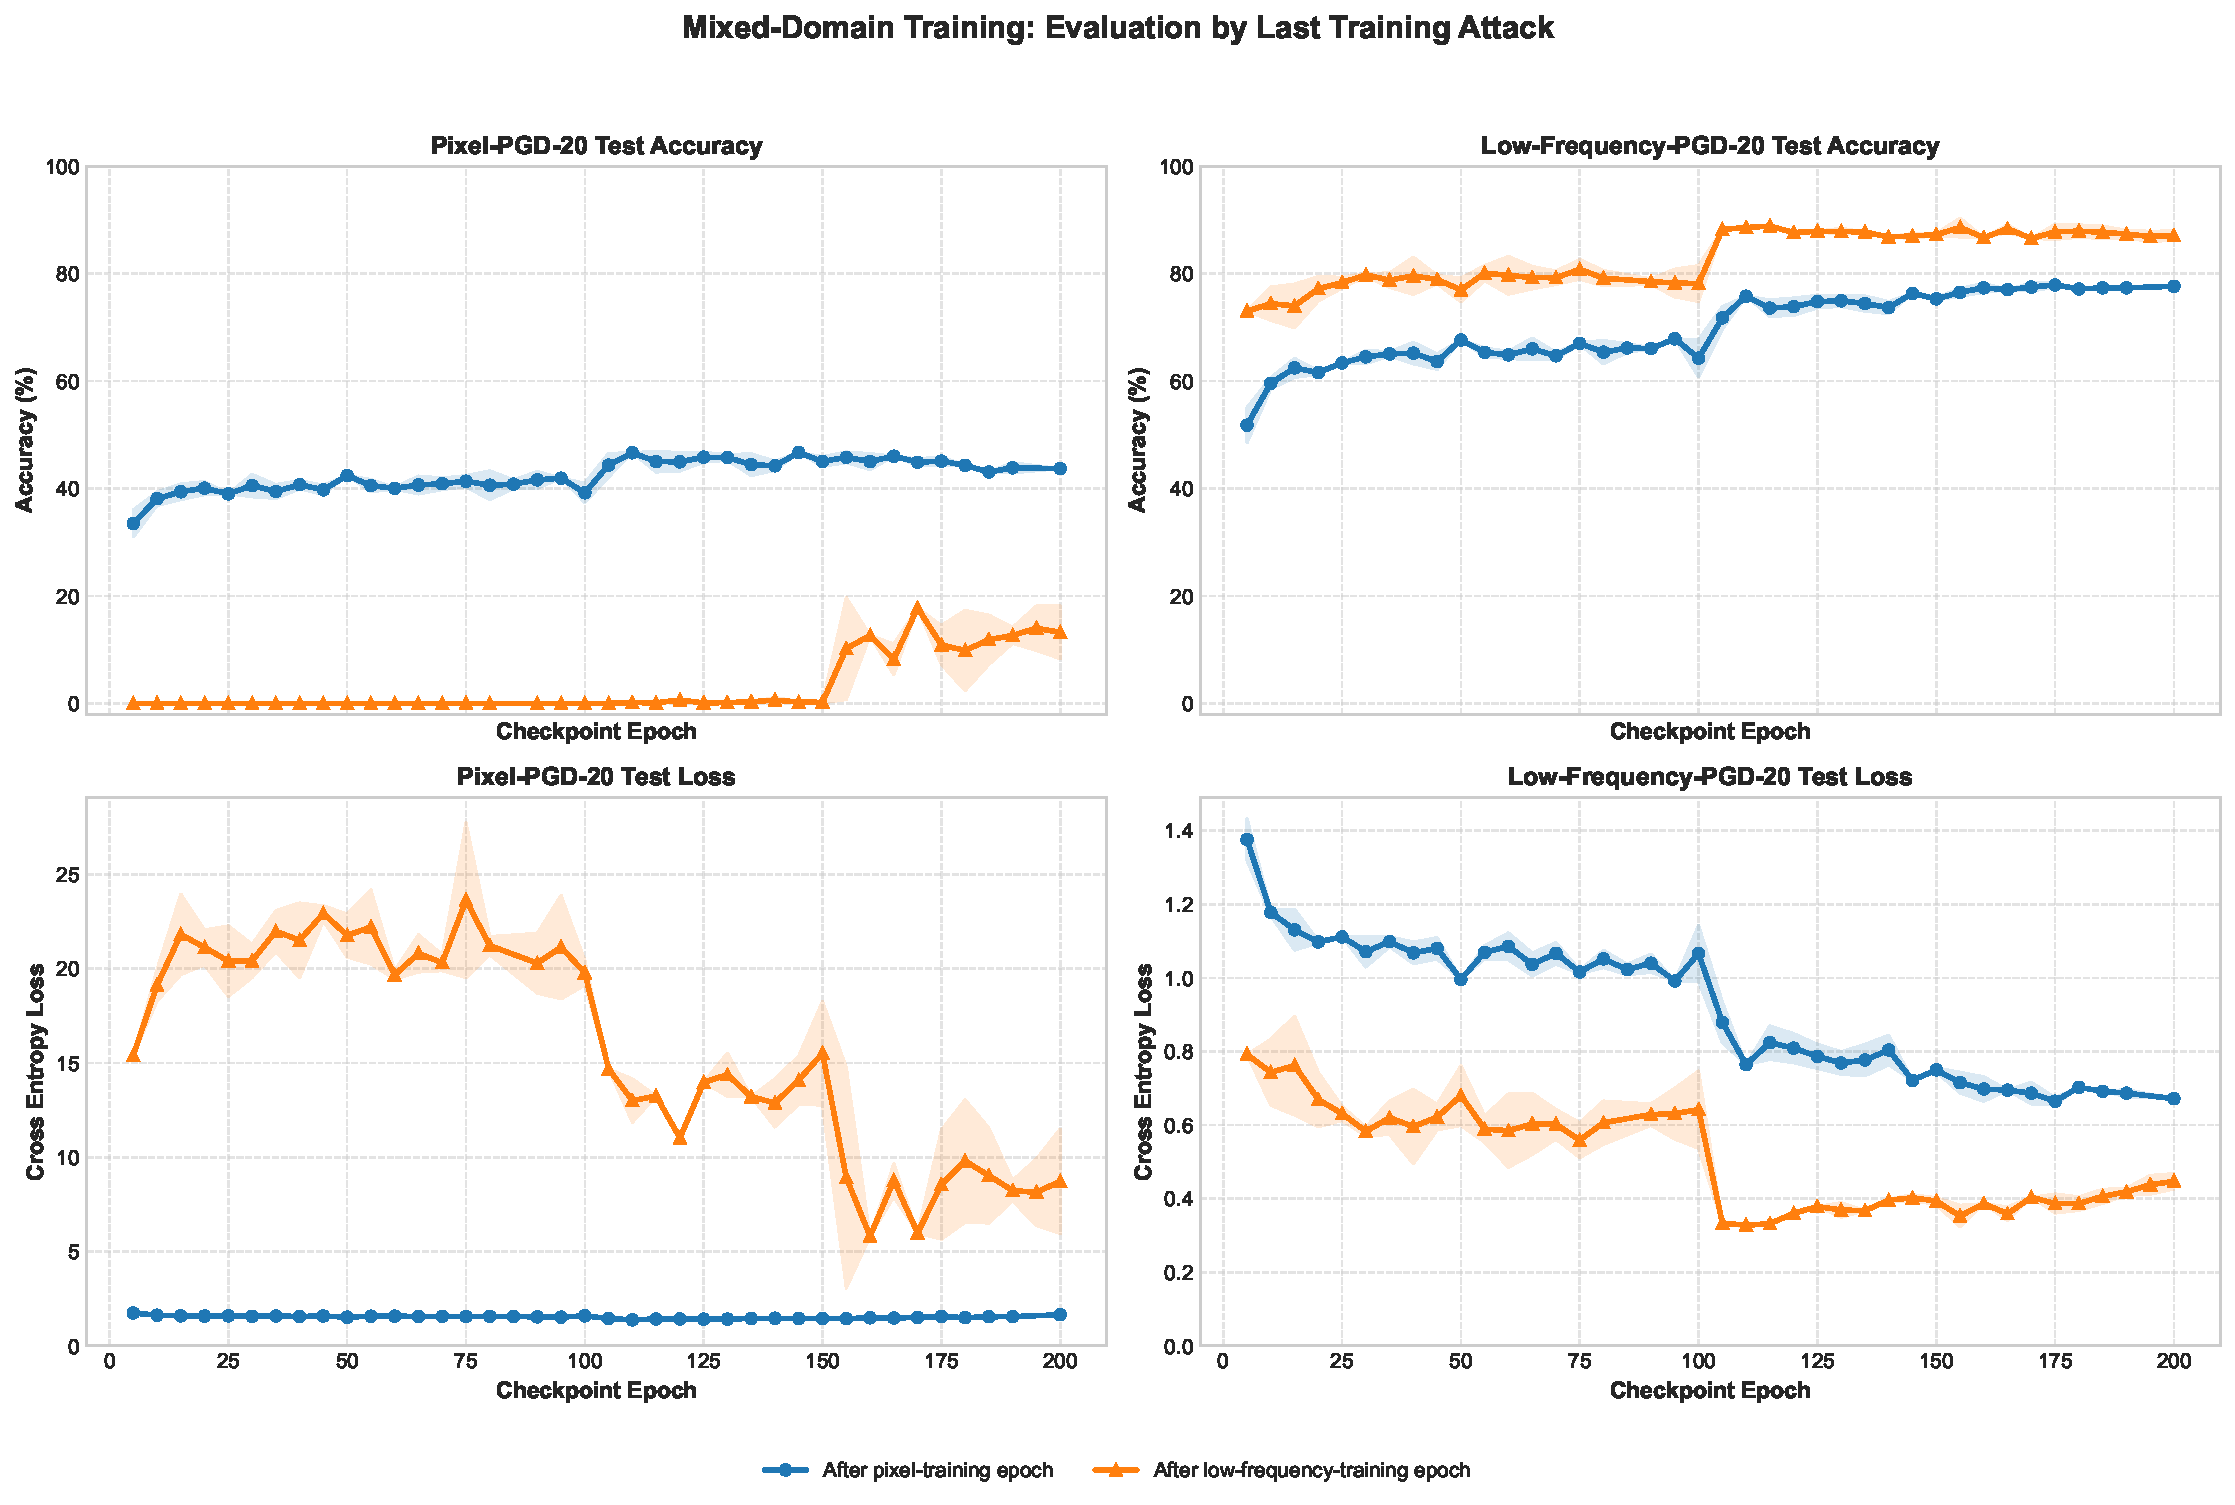
\includegraphics[width=\linewidth]{mixed-domain/overall/mdo_eval_grouped.pdf}
  \caption{Mixed-domain checkpoint evaluation grouped by the attack used in
  the final training epoch before each checkpoint. Each point averages the
  seeds with the indicated preceding domain. Group sizes vary from one to
  five; shaded bands show sample standard deviation when at least two seeds
  contribute. Singleton groups have zero-width bands, and epochs with no
  contributing seeds are omitted. Pixel-PGD-20 robustness is consistently
  much higher
  after pixel-training epochs, whereas low-frequency-PGD-20 robustness is
  higher after low-frequency-training epochs. This schedule-linked recency
  effect reveals alternating domain-specialized states rather than stable
  simultaneous robustness.}
  \label{fig:mixed-eval-grouped}
\end{figure}

\FloatBarrier
\section{Discussion}
\label{sec:discussion}

Pixel-only training achieves the highest final pixel and joint accuracy,
while low-frequency-only training achieves the highest final clean and
low-frequency accuracy. Epoch-wise mixing does not provide stable robustness
across both evaluated attacks.

\subsection{Interpretation}
The results are consistent with the hypothesis: the training attack changes
the timing and shape of measured robustness. The small low-frequency accuracy
gap does not imply that every
measure remains stable: low-frequency test loss rises after its epoch-105
minimum.

These experiments show how robustness differs across the training conditions,
but they do not determine why these differences occur. Possible explanations
include which frequency components the models learn to use, how the attack
updates affect learning, and whether training against one attack reduces
robustness to the other. Further controlled experiments would be needed to
distinguish these explanations. In particular, the
mixed-domain results do not show that epoch-wise mixing mitigates robust
overfitting, and the high low-frequency accuracy still needs stronger
matched-domain attack checks.

\subsection{Practical implications}
The control condition suggests that the final checkpoint can be substantially
worse than an earlier checkpoint under pixel-PGD-20, reinforcing the practical
importance of validation-based early stopping. The low-frequency-only condition
also illustrates that strong performance under a restricted perturbation model
does not imply observed robustness to pixel PGD without a frequency
restriction. For a deployment
claim, model selection and evaluation must match the intended threat model.

A concrete protocol is to reserve a validation split before training, evaluate
every candidate checkpoint under the intended finite-step attack configuration,
and select the checkpoint using a predeclared validation criterion. For a
pixel-only deployment, that criterion can be pixel-PGD validation accuracy;
for a multi-threat deployment, it should be a predeclared joint criterion,
such as per-example joint accuracy under the chosen attacks. The
minimum of the two aggregate accuracies can overstate this joint accuracy
when the attacks trick different examples. The test set should then be evaluated
once
for the selected checkpoint, with each component attack reported separately.

\section{Limitations}
\label{sec:limitations}
\begin{itemize}
  \item \textbf{Attack evaluation.} PGD-20 with one reported configuration is
  not a proof of robustness. More iterations, additional restarts, adaptive
  attacks, and broader attack suites may change measured accuracy. The
  stronger-attack diagnostic covers only two pixel-only checkpoints; the
  low-frequency and mixed-domain results have no comparable check.
  \item \textbf{Meaning of joint accuracy.} Joint accuracy tests two separately
  generated adversarial examples per image. It does not establish worst-case
  accuracy over the full threat set.
  \item \textbf{Threat sets and attack updates.} With the same $\linf$ budget, the
  final low-frequency perturbations lie within the pixel threat set despite
  clipping-induced spectral leakage. Frequency restriction and the different
  attack update rules are not isolated experimentally.
  \Needspace{4\baselineskip}
  \item \textbf{Scope.} The study uses one architecture, CIFAR-10, a single
  cutoff ($8$), one 200-epoch schedule, and five seeds. It does not establish
  generality across data sets, architectures, budgets, or frequency bands.
  \item \textbf{Epoch-wise mixing.} The study selects one attack per epoch.
  It does not test mixing within batches or individual examples, enforce an
  equal number of epochs for each attack, select the worst-case attack per
  example, or measure gradient interactions between attacks.
  \item \textbf{Model selection.} Checkpoint peaks are found on the test set
  for descriptive analysis; they are not validation-selected estimates of
  deployable early-stopping performance.
  \item \textbf{Reproducibility.} Saved checkpoints and TensorBoard logs
  record the training conditions and trajectories, but exact cloud software
  versions and command histories were not retained. Bitwise reproduction
  across environments has not been established.
\end{itemize}

\section{Conclusion}
\label{sec:conclusion}
Across five seeds, pixel-only training reproduced robust overfitting under
pixel-PGD-20: mean pixel robustness peaked at 51.22\% at epoch 105 and fell
by 8.56 percentage points by epoch 200. Low-frequency-only training instead
maintained 92.70\% final low-frequency robustness with a 0.05-point
best-versus-final decline, while exhibiting 0.00\% measured pixel and
joint accuracy. Once-per-epoch mixed-domain training did not produce
stable simultaneous robustness; its pixel robustness was strongly associated
with the most recent training domain. These findings apply to PreActResNet-18 on CIFAR-10 with the selected DCT
cutoff and attack settings. Future work should compare epoch-wise mixing
with mixing within batches or individual examples, using validation-based
checkpoint selection and a broader attack evaluation.

\section*{Acknowledgments}
The author gratefully acknowledges Nicholas Tran for mentorship and
constructive feedback on the research design, analysis, and presentation.

\section*{Reproducibility and Artifact Map}
\addcontentsline{toc}{section}{Reproducibility and Artifact Map}
The source code, evaluation results, diagnostic checks, and reproduction
instructions are available at
\url{https://github.com/ItsKaiwenDu/Robust-Overfitting}.
The main files and directories are organized as follows:
\begin{itemize}
  \item \texttt{scripts/train.py}: adversarial training, checkpoints, seeded
  mixed-domain scheduling, and TensorBoard logging;
  \item \texttt{scripts/dct\_pgd.py}: DCT, masking, projection, and
  low-frequency PGD implementation;
  \item \texttt{scripts/evaluate.py}: checkpoint evaluation under clean,
  pixel-PGD-20, low-frequency-PGD-20, and joint metrics;
  \item \texttt{scripts/plot\_results.py}: per-seed and overall plots;
  \item \texttt{scripts/run\_report\_checks.py}: DCT, perturbation-budget,
  clipping-leakage, and attack-strength diagnostics;
  \item \texttt{report/checks/}: saved diagnostic results supporting Appendix~\ref{app:checks};
  \item \texttt{report/<condition>/overall/}: five-seed mean and
  standard-deviation checkpoint summaries and aggregate figures.
\end{itemize}
All 600 checkpoints from the three training conditions are available on
\href{https://huggingface.co/KaiwenDu/robust-overfitting-checkpoints}{Hugging Face},
organized by condition, seed, and epoch.

\FloatBarrier
\appendix
\setcounter{topnumber}{5}
\setcounter{bottomnumber}{5}
\setcounter{totalnumber}{5}
\renewcommand{\topfraction}{0.9}
\renewcommand{\bottomfraction}{0.8}
\renewcommand{\textfraction}{0.1}
\renewcommand{\floatpagefraction}{0.7}
\section{Per-seed Results}
\label{app:per-seed}
\Cref{tab:per-seed-pixel,tab:per-seed-low-frequency,tab:per-seed-mixed}
provide the seed-level counterpart to the aggregate trajectories. The reported
metric is pixel-PGD-20 accuracy for the pixel-only and mixed-domain conditions
and low-frequency-PGD-20 accuracy for the low-frequency-only condition. Peak
epochs use the first evaluated epoch attaining the seed-level maximum. The
mixed-domain gaps remain schedule-confounded and are included to make the
seed-level variation transparent rather than as standalone estimates of
conventional robust overfitting.

\begin{table}[!htbp]
\centering
\caption{Pixel-PGD-20 accuracy by seed for pixel-only training.
Accuracies are percentages; gaps are percentage points.}
\label{tab:per-seed-pixel}
\begin{tabular*}{\linewidth}{@{\extracolsep{\fill}}lrrrr@{}}
\toprule
Seed & Peak epoch & Peak accuracy & Epoch-200 accuracy & Gap \\
\midrule
42 & 105 & 51.30 & 42.57 & 8.73 \\
43 & 105 & 51.45 & 42.56 & 8.89 \\
44 & 105 & 51.18 & 42.88 & 8.30 \\
45 & 105 & 51.41 & 42.89 & 8.52 \\
46 & 105 & 50.76 & 42.40 & 8.36 \\
\bottomrule
\end{tabular*}
\end{table}

\begin{table}[!htbp]
\centering
\caption{Low-frequency-PGD-20 accuracy by seed for low-frequency-only
training. Accuracies are percentages; gaps are percentage points.}
\label{tab:per-seed-low-frequency}
\begin{tabular*}{\linewidth}{@{\extracolsep{\fill}}lrrrr@{}}
\toprule
Seed & Peak epoch & Peak accuracy & Epoch-200 accuracy & Gap \\
\midrule
42 & 200 & 92.94 & 92.94 & 0.00 \\
43 & 195 & 92.79 & 92.70 & 0.09 \\
44 & 200 & 92.99 & 92.99 & 0.00 \\
45 & 195 & 92.51 & 92.33 & 0.18 \\
46 & 170 & 92.65 & 92.53 & 0.12 \\
\bottomrule
\end{tabular*}
\end{table}

\begin{table}[!htbp]
\centering
\caption{Pixel-PGD-20 accuracy by seed for mixed-domain training.
Accuracies are percentages; gaps are percentage points. These raw gaps
are confounded by the epoch-level attack schedule.}
\label{tab:per-seed-mixed}
\begin{tabular*}{\linewidth}{@{\extracolsep{\fill}}lrrrr@{}}
\toprule
Seed & Peak epoch & Peak accuracy & Epoch-200 accuracy & Gap \\
\midrule
42 & 160 & 46.16 & 43.71 & 2.45 \\
43 & 115 & 47.79 & 15.93 & 31.86 \\
44 & 155 & 46.83 & 5.96 & 40.87 \\
45 & 125 & 46.27 & 14.58 & 31.69 \\
46 & 130 & 45.58 & 16.48 & 29.10 \\
\bottomrule
\end{tabular*}
\end{table}

\FloatBarrier
\Needspace{14\baselineskip}
\section{Mixed-Domain Schedules}
\label{app:schedules}
The complete schedules were read from the \texttt{attack\_domain\_schedule}
metadata stored in each epoch-200 checkpoint. Every schedule has 200 entries,
matches the saved final attack domain, and uses the recorded cutoff of $8$.
\Cref{tab:mixed-schedules} reports the realized balance. The schedules are
near-balanced but not constrained to be exactly balanced, as intended by the
independent seeded random choice. All five runs ended epoch 85 with pixel
training, whereas only seed 42 did so at epoch 200.

\begin{table}[!htbp]
\centering
\caption{Realized mixed-domain attack schedules extracted from saved
epoch-200 checkpoint metadata.}
\label{tab:mixed-schedules}
\begin{tabular*}{\linewidth}{@{\extracolsep{\fill}}lrrll@{}}
\toprule
Seed & Pixel epochs & Low-frequency epochs & Epoch-85 domain & Epoch-200 domain \\
\midrule
42 & 113 & 87 & Pixel & Pixel \\
43 & 106 & 94 & Pixel & Low-frequency \\
44 & 101 & 99 & Pixel & Low-frequency \\
45 & 98 & 102 & Pixel & Low-frequency \\
46 & 100 & 100 & Pixel & Low-frequency \\
\bottomrule
\end{tabular*}
\end{table}

\FloatBarrier
\section{Attack-Strength and Implementation Checks}
\label{app:checks}
The attack checks use a fixed, approximately class-balanced 256-image subset
of the CIFAR-10 test set (selection seed 20260912); the DCT algebra checks use
random tensors. These are diagnostic checks only; the primary results remain the full-test-set,
single-restart PGD-20 measurements reported in \cref{sec:results}.

\paragraph{DCT and perturbation checks.}
On eight random three-channel $32\times32$ tensors, the maximum absolute DCT--inverse-DCT
round-trip error was $1.11\times10^{-5}$. Projecting these tensors to the
$8\times8$ mask left an out-of-mask energy fraction of at most
$2.53\times10^{-12}$. We then generated low-frequency PGD-20 examples with the
low-frequency-only seed-42 epoch-200 checkpoint. Before final image clipping,
the maximum out-of-mask energy fraction was $3.36\times10^{-12}$; after
clipping, the mean, 95th-percentile, and maximum fractions were 0.70\%,
4.75\%, and 17.56\%, respectively. The maximum final perturbation norm was
$0.03137258$, equal to $8/255$ to floating-point precision. Thus projection
and budget enforcement behave as intended, while final image clipping creates
some high-frequency leakage.

\begin{table}[!htbp]
\centering
\caption{Pixel attack-strength diagnostic for pixel-only seed 42 on a fixed
256-image test subset. PGD-20 uses one random start. PGD-50 uses three random
starts and retains, for each image, the final candidate with the highest
cross-entropy loss. Accuracy is in percent. $\Delta$ is PGD-50 accuracy minus
PGD-20 accuracy, in percentage points.}
\label{tab:attack-strength}
\begin{tabular*}{\linewidth}{@{\extracolsep{\fill}}lrrrr@{}}
\toprule
Checkpoint & PGD-20 & PGD-50 & $\Delta$ & PGD-50 loss \\
\midrule
Epoch 105 & 49.22 & 48.83 & $-0.39$ & 1.319 \\
Epoch 200 & 38.67 & 38.28 & $-0.39$ & 3.529 \\
\bottomrule
\end{tabular*}
\end{table}

The stronger attack reduces accuracy by one example out of 256 at each
checkpoint and raises mean cross-entropy loss from 1.312 to 1.319 at epoch 105
and from 3.486 to 3.529 at epoch 200. This small diagnostic does not reveal a
large PGD-20 weakness in the selected control checkpoints, but it does not
substitute for multiple full-test restarts, adaptive attacks, or a broader
attack suite.

\FloatBarrier
\section{Mixed-Domain Training Dynamics}
\label{app:mixed-training}
\Cref{fig:mixed-training} complements the checkpoint evaluations in
\cref{sec:mixed-results} with the measurements recorded during training.

\begin{figure}[htbp]
  \centering
  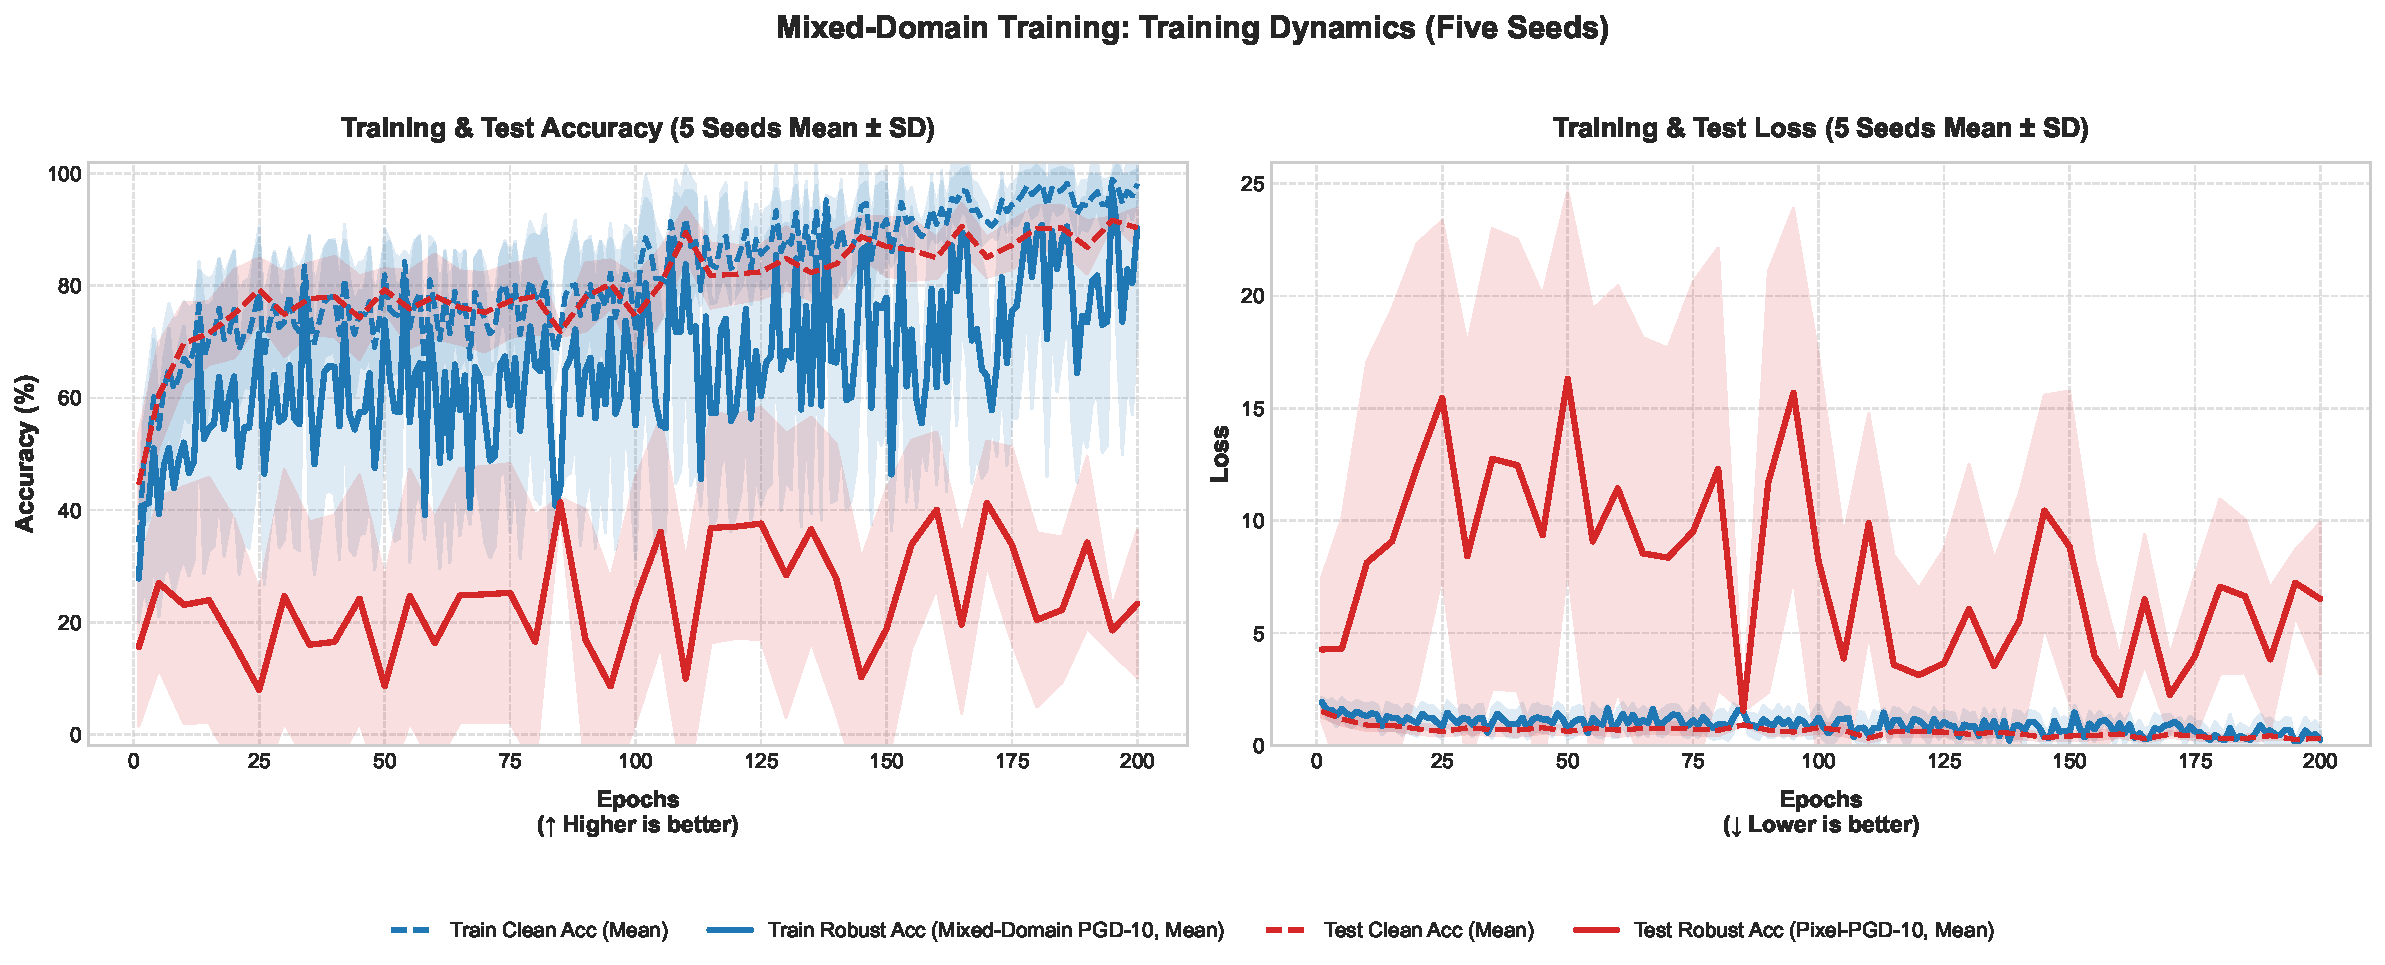
\includegraphics[width=\linewidth]{mixed-domain/overall/mdo_train.pdf}
  \caption{Mixed-domain training dynamics across five seeds; shaded bands
  show one sample standard deviation. Training robustness is measured against
  the PGD-10 attack selected for each seed and epoch. Test robustness is always
  measured against pixel-PGD-10. The training curves therefore combine results
  from different attacks and do not represent joint accuracy.}
  \label{fig:mixed-training}
\end{figure}

\clearpage
\begin{thebibliography}{99}

\bibitem{goodfellow2015}
I. J. Goodfellow, J. Shlens, and C. Szegedy.
\newblock \href{https://arxiv.org/abs/1412.6572}{Explaining and Harnessing Adversarial Examples}.
\newblock In \emph{International Conference on Learning Representations
(ICLR)}, 2015.

\bibitem{madry2018}
A. Madry, A. Makelov, L. Schmidt, D. Tsipras, and A. Vladu.
\newblock \href{https://arxiv.org/abs/1706.06083}{Towards Deep Learning Models Resistant to Adversarial Attacks}.
\newblock In \emph{International Conference on Learning Representations
(ICLR)}, 2018.

\bibitem{rice2020}
L. Rice, E. Wong, and J. Z. Kolter.
\newblock \href{https://proceedings.mlr.press/v119/rice20a.html}{Overfitting in Adversarially Robust Deep Learning}.
\newblock In \emph{Proceedings of the 37th International Conference on Machine
Learning}, PMLR 119:8093--8104, 2020.

\bibitem{yu2022}
C. Yu, B. Han, L. Shen, J. Yu, C. Gong, M. Gong, and T. Liu.
\newblock \href{https://proceedings.mlr.press/v162/yu22b.html}{Understanding Robust Overfitting of Adversarial Training and Beyond}.
\newblock In \emph{Proceedings of the 39th International Conference on Machine
Learning}, PMLR 162:25595--25610, 2022.

\bibitem{guo2020}
C. Guo, J. S. Frank, and K. Q. Weinberger.
\newblock \href{https://proceedings.mlr.press/v115/guo20a.html}{Low Frequency Adversarial Perturbation}.
\newblock In \emph{Proceedings of the 35th Uncertainty in Artificial
Intelligence Conference}, PMLR 115:1127--1137, 2020.

\bibitem{chen2022}
Y. Chen, Q. Ren, and J. Yan.
\newblock \href{https://proceedings.neurips.cc/paper_files/paper/2022/hash/022abe84083d235f7572ca5cba24c51c-Abstract-Conference.html}{Rethinking and Improving Robustness of Convolutional Neural Networks:
A Shapley Value-based Approach in Frequency Domain}.
\newblock In \emph{Advances in Neural Information Processing Systems 35}, 2022.

\bibitem{bu2023}
Q. Bu, D. Huang, and H. Cui.
\newblock \href{https://openaccess.thecvf.com/content/ICCV2023/html/Bu_Towards_Building_More_Robust_Models_with_Frequency_Bias_ICCV_2023_paper.html}{Towards Building More Robust Models with Frequency Bias}.
\newblock In \emph{Proceedings of the IEEE/CVF International Conference on
Computer Vision}, pages 4402--4411, 2023.

\bibitem{tramer2019}
F. Tram\`er and D. Boneh.
\newblock \href{https://proceedings.neurips.cc/paper_files/paper/2019/hash/5d4ae76f053f8f2516ad12961ef7fe97-Abstract.html}{Adversarial Training and Robustness for Multiple Perturbations}.
\newblock In \emph{Advances in Neural Information Processing Systems 32}, 2019.

\bibitem{maini2020}
P. Maini, E. Wong, and J. Z. Kolter.
\newblock \href{https://proceedings.mlr.press/v119/maini20a.html}{Adversarial Robustness Against the Union of Multiple Perturbation
Models}.
\newblock In \emph{Proceedings of the 37th International Conference on Machine
Learning}, PMLR 119:6640--6650, 2020.

\bibitem{xie2026}
M. Xie, Y. He, and M. Fang.
\newblock \href{https://arxiv.org/abs/2606.17540}{TaFD: Threat-Aware Frequency Decoupling for Adversarial Robustness
against Heterogeneous Attacks}.
\newblock arXiv:2606.17540 [cs.CV], 2026.

\bibitem{he2016}
K. He, X. Zhang, S. Ren, and J. Sun.
\newblock \href{https://doi.org/10.1007/978-3-319-46493-0_38}{Identity Mappings in Deep Residual Networks}.
\newblock In \emph{Computer Vision: ECCV 2016}, pages 630--645, 2016.

\bibitem{krizhevsky2009}
A. Krizhevsky.
\newblock \href{https://www.cs.toronto.edu/~kriz/cifar.html}{Learning Multiple Layers of Features from Tiny Images}.
\newblock Technical report, University of Toronto, 2009.

\end{thebibliography}

\end{document}
